\documentclass[10pt]{report}
\usepackage{lingmacros}
\usepackage[normalem]{ulem}
%  Title Formatting 
\usepackage{titlesec}
% Removes paragraph indenting
\usepackage{parskip} 

% Font
\usepackage{tgpagella}

% Inline code
\usepackage{listings, lstautogobble}

\usepackage[labelfont=bf, labelsep=period]{caption}
\usepackage{graphicx}
\graphicspath{ {./images/} }

% Makes citations superscript
\usepackage[superscript,biblabel]{cite}
\usepackage{url}
\urlstyle{same}

\titleformat{\chapter}[block]
{\normalfont\huge\bfseries}{\thechapter.}{1em}{\Huge}
\titlespacing*{\chapter}{0pt}{-19pt}{0pt}

\lstset{language=Java,
	showstringspaces=false,
	breaklines=true,
	frameround=ffff,
	frame=single,
	autogobble=true
}

\begin{document}
	\begin{titlepage}
		\begin{center}
			\Large
			\textbf{Procedural Generation Using Noise}
			
			\vspace{1.5cm}
			\normalsize
			\textbf{Michael Li}
			
			\vfill
			
			\textbf{DRAFT 1.0.1}
			
			\uline{Dr.Dianne Hansford \hfill Director}
			\vspace{1.5cm}
			
			\uline{Dr.Yoshihiro Kobayashi \hfill Second Committee Member}
			
			\vspace{3cm}
			
			
\includegraphics[scale=.5]{asu_barretthonors_horiz_rgb_maroongold_600ppi}
			
			\vspace{1.5cm}
			Ira A. Fulton Schools of Engineering
			
			School of Computing, Informatics, and Decision Systems Engineering
			
			Spring 2021
			
		\end{center}
	\end{titlepage}
	
	\chapter*{Abstract}
	
	\addcontentsline{toc}{chapter}{Abstract}
	Procedural Content Generation is a method of creating data algorithmically, often using stochastic models. These methods can be used to generate complex environments as opposed to manually creating environments by hand or by using photogrammetric techniques. Procedural generation can use a variety of techniques to achieve a stochastic or partially stochastic goal, including methods such as fractals,  noise, deep learning as examples.
	
	\clearpage
	
	\tableofcontents
	
	\clearpage
	
	\let\clearpage\relax
	\chapter{Introduction}
	
		This paper surveys various methods of procedural generation and their applications in generating geological formations. While procedural generated content can vary from terrain to creatures and stories, the focus of this paper is primarily on terrain and more specifically geological formations. One of the most famous cases of this procedural generation for geological formations is in Minecraft, which implements a modified version of Perlin noise in order to generate all of its worlds. Other examples can include games such as the Elder Scrolls II: Daggerfall, which employed various forms of procedural generation to determine the location of non-player characters, the layout of dungeons, as well as the terrain itself. In more complex cases, procedural generation can be used to create fake histories, with the more well known example of Dwarf Fortress. However, procedural generation's applications are not only limited to games. In the creation of the Lord of the Rings movies, procedural generation was applied to help create the many different forms of orcs in the movie, as well as ensuring that each orc was able to be animated. While procedural generation is often described as being stochastic, in reality it is not entirely so. The majority of the techniques used for procedural generation include some level of user control, as well as a specified input to use as a starting point for the equation. This input, known as a seed is transformed through code to create the output, in this case geological formations.
		
		The main topic that this paper will cover is the mapping of geological formations. While this can be done through height maps, which are black and white, or colored maps where the colors or intensity of the black/white indicate the height of each point. This acts as a two dimensional representation of the terrain, although it has difficulty in representing structures that have undersides.
		
		\section{Influences}
		
		Procedural generation has a history rooted in math, particularly the work involving Brownian motion as well as fractals. Before the development of other procedural generation techniques, some basic procedural generation techniques were used in the 1980s. One of the earliest usages of procedural generation was in Rogue. This initial attempt at generating a dungeon in a random manner addressed some of the differences between procedural generation and purely random generation. Rogue addressed this issue through procedural generation, 1ref using a three by three grid in order to generate the layout of the level, with hallways randomly connecting the rooms. These rooms would have a variable size in order to increase the variety of levels producible by the algorithm. This technique in particular, was created to address the memory constraints of computers at the time, as even with this more mathematical and less memory  intensive approach, levels would need to be cleared from memory when moving on to the next one.
		% 1ref % Michael Toy, G.W. Rogue; Epyx: San Francisco, CA, USA, 1980
		% Craddock, David L (August 5, 2015). "Chapter 2: "Procedural Dungeons of Doom: Building Rogue, Part 1"". In Magrath, Andrew (ed.). Dungeon Hacks: How NetHack, Angband, and Other Roguelikes Changed the Course of Video Games. Press Start Press. ISBN 978-0-692-50186-3.
		
		
		\section{Overview and Definitions}
		
		Procedural generation is often dependent on the use of random numbers, which has varying methods of generation in a computer. There are two strategies for the generation of these random numbers, producing the numbers non-deterministically through the use of unpredictable physical processes, and computing numbers deterministically using an algorithm. While the determination of this random number is not important for procedural generation, as the necessity of security is less, procedural generation algorithms follow the same methodology as the deterministic random bit generators. In procedural generation, a seed is a random number where the rest of the generation will begin from. This ensures regularity to the procedural generation, by allowing for the algorithm used to have repeatable results. By taking an input seed, it will be modified using an equation to obtain the output, possibly using additional random numbers created after the original seed.
		% citation: https://nvlpubs.nist.gov/nistpubs/SpecialPublications/NIST.SP.800-90Ar1.pdf
		
		One of the applications of these random numbers is through the creation of noise. Noise in this application refers to the spreading of values across a coordinate plane. Lattice gradient noise is a commonly used and widespread form of noise. One of the most well known applications of this is Perlin noise, notably developed for Tron, but also applied in games like Minecraft. This form of procedural generation works off of the premise of an integer lattice - a regularly spaced array of points in a square array\cite{integer-lattice}. Pseudo-random numbers are generated and evenly distributed across this lattice, then a low-pass filter is applied in order to smooth the edges between each of these points. The low pass filter's effect is just creating the gradation between each of the lattice points. The result is an image such as this one.
		
		****INSERT IMAGE HERE ****

		Fractal landscapes is another approach at procedural generation. Fractal geometry being applied to landscapes began with studies of map data and research on the similarities between fractals and the data. Fractals prove as a relevant approach to representing geographical data due to the self similarity and the subdivision of space, made easier by fractal surfaces. This provides a method of predicting or as an initial hypothesis for landscapes in study. The technique works primarily from the subdivision of space combined with random numbers for each of the vertices created from the subdivision. Similarly to Perlin noise, this technique often utilizes a seed random number to start from, in order to make the results reproducible. However, while fractals are very computationally efficient, the parameter that makes this seed is very sensitive to change. Very small changes will completely change the features of a map designed this way.
		% https://www.sciencedirect.com/science/article/pii/0169555X9390022T
		% http://paulbourke.net/fractals/noise/
		% https://www.playfuljs.com/realistic-terrain-in-130-lines/
		% https://www.tandfonline.com/doi/abs/10.1111/j.1467-8306.1987.tb00158.x
		% https://www.sciencedirect.com/science/article/pii/0169555X9390022T
		Another method of generating terrain revolves around the use of cellular automata. define cellular automata. Cellular automata works on a grid of cells, similarly to how noise is mapped, but instead of having a continuous value, the cells in this approach only have binary values, or similar. This approach relies of having the information of neighbors and the states of their neighbors to determine surrounding cells to then modify their states. This can be used in conjunction with a tiling system in order to procedurally generate worlds, albeit with pre-determined cells for usage.
		% https://natureofcode.com/book/chapter-7-cellular-automata/
		% https://www.um.edu.mt/library/oar/bitstream/123456789/22895/1/Cellular_automata_for_real-time_generation_of.pdf
		Representing the data generated procedurally is another task with a variety of solutions. Some of these methods include pixel based methods, polygons and voxels. One common, simplistic way to represent the data generated is to use ascii characters, or other types of two dimensional data such as colored pixels in order to convey the scene that is being represented. In the case of Dwarf Fortress, the use of color and text symbols is used to represent the graphics of the game, with examples such as letters representing animals, or other characters representing terrain elements. 
		
		Another of the ways of representing three-dimensional objects is through the use of polygon meshes. These are created through polygons (typically triangles) joined by at least two vertices. These polygons are then represented by the coordinates of the vertices that compose them, while the space between the vertices acts as the viewable portion.
		
		In contrast to polygons representing faces of a geometry, voxels represent a value on a in space. Voxels are represented by their position relative to other voxels, allowing for easier representation of layers of geometry. An example of this voxel rendering can be found in the voxel space rendering engine, used for early flight simulator games. This used pre-generated height and color maps to determine which pixels would be visible on the screen, and at what height. The result is a fairly efficient method of rendering the player's perspective, at the cost of being unable to have more complex landscapes. In modern voxel based approaches, more complicated methods are used in order to render complex landscapes accurately.
		
	\vspace{10pt}
	\let\clearpage\relax
	\chapter{Historical Usage}
		
		Perlin noise was developed for use in the movie industry, although it later became a foundation for many other procedural generation algorithms as it provided a lot of control as well as randomness to be used. It was developed in 1983 for use in the sci-fi movie Tron, to map textures onto computer generated surfaces for visual effects. Perlin noise has been used for many different visual elements, ranging from the texture creation it was created for to particle effects such as fire, smoke and clouds, as well as landscapes and geological features. It has a variety of uses due to its ability to create a naturalistic appearance.
		
		As previously described, Perlin noise is a form of lattice based gradient noise. This usually generates noise from an input seed, and creates a gradient of pseudo-random, regularly spaced points from this. Then, in order to create the transitions between these points in space, a gradient/slope is associated with each of these points in space.
		% https://dl.acm.org/doi/10.1145/325165.325247
		
		% cellular automata
		
		% fractal geometry
		
		% branching stuff
		
		% simple if statements with some level of randomness
		
	\vspace{10pt}
	\let\clearpage\relax
	\chapter{Image Based Methods}
	
		Some of the other uses of height maps include the voxel space rendering system, using voxel raster graphics to display three-dimensional geometry with low memory and processing requirements. This was developed in the early 90's, involving a height and color map to position the pixels on the screen. While this technique was not historically used with noise generating algorithms, the rendering system fits the requirements for the use of techniques such as two-dimensional Perlin noise. At the time, displaying complex height-maps in three-dimensions was difficult computationally, and the voxel space technique allowed this to happen. 
		
		The voxel space rendering engine originally utilized a pre-made height and color map to render from. This, combined with a tiling effect and knowledge of the field-of-view of the user's position allowed for a simplified three-dimensional rendering system. Starting from the furthest position to guarantee occlusion, a line on the map is determined in the triangular field of view. This is scaled with perspective projection, and a vertical line is drawn at every point on the screen from the section of the color map. The height of the vertical line is determined from the height drawn from the two-dimensional height map. Then, this is repeated until the entire field-of-view is drawn. This technique can be seen in Figure 1. 
		
		\begin{minipage}{\textwidth}
			\centering
			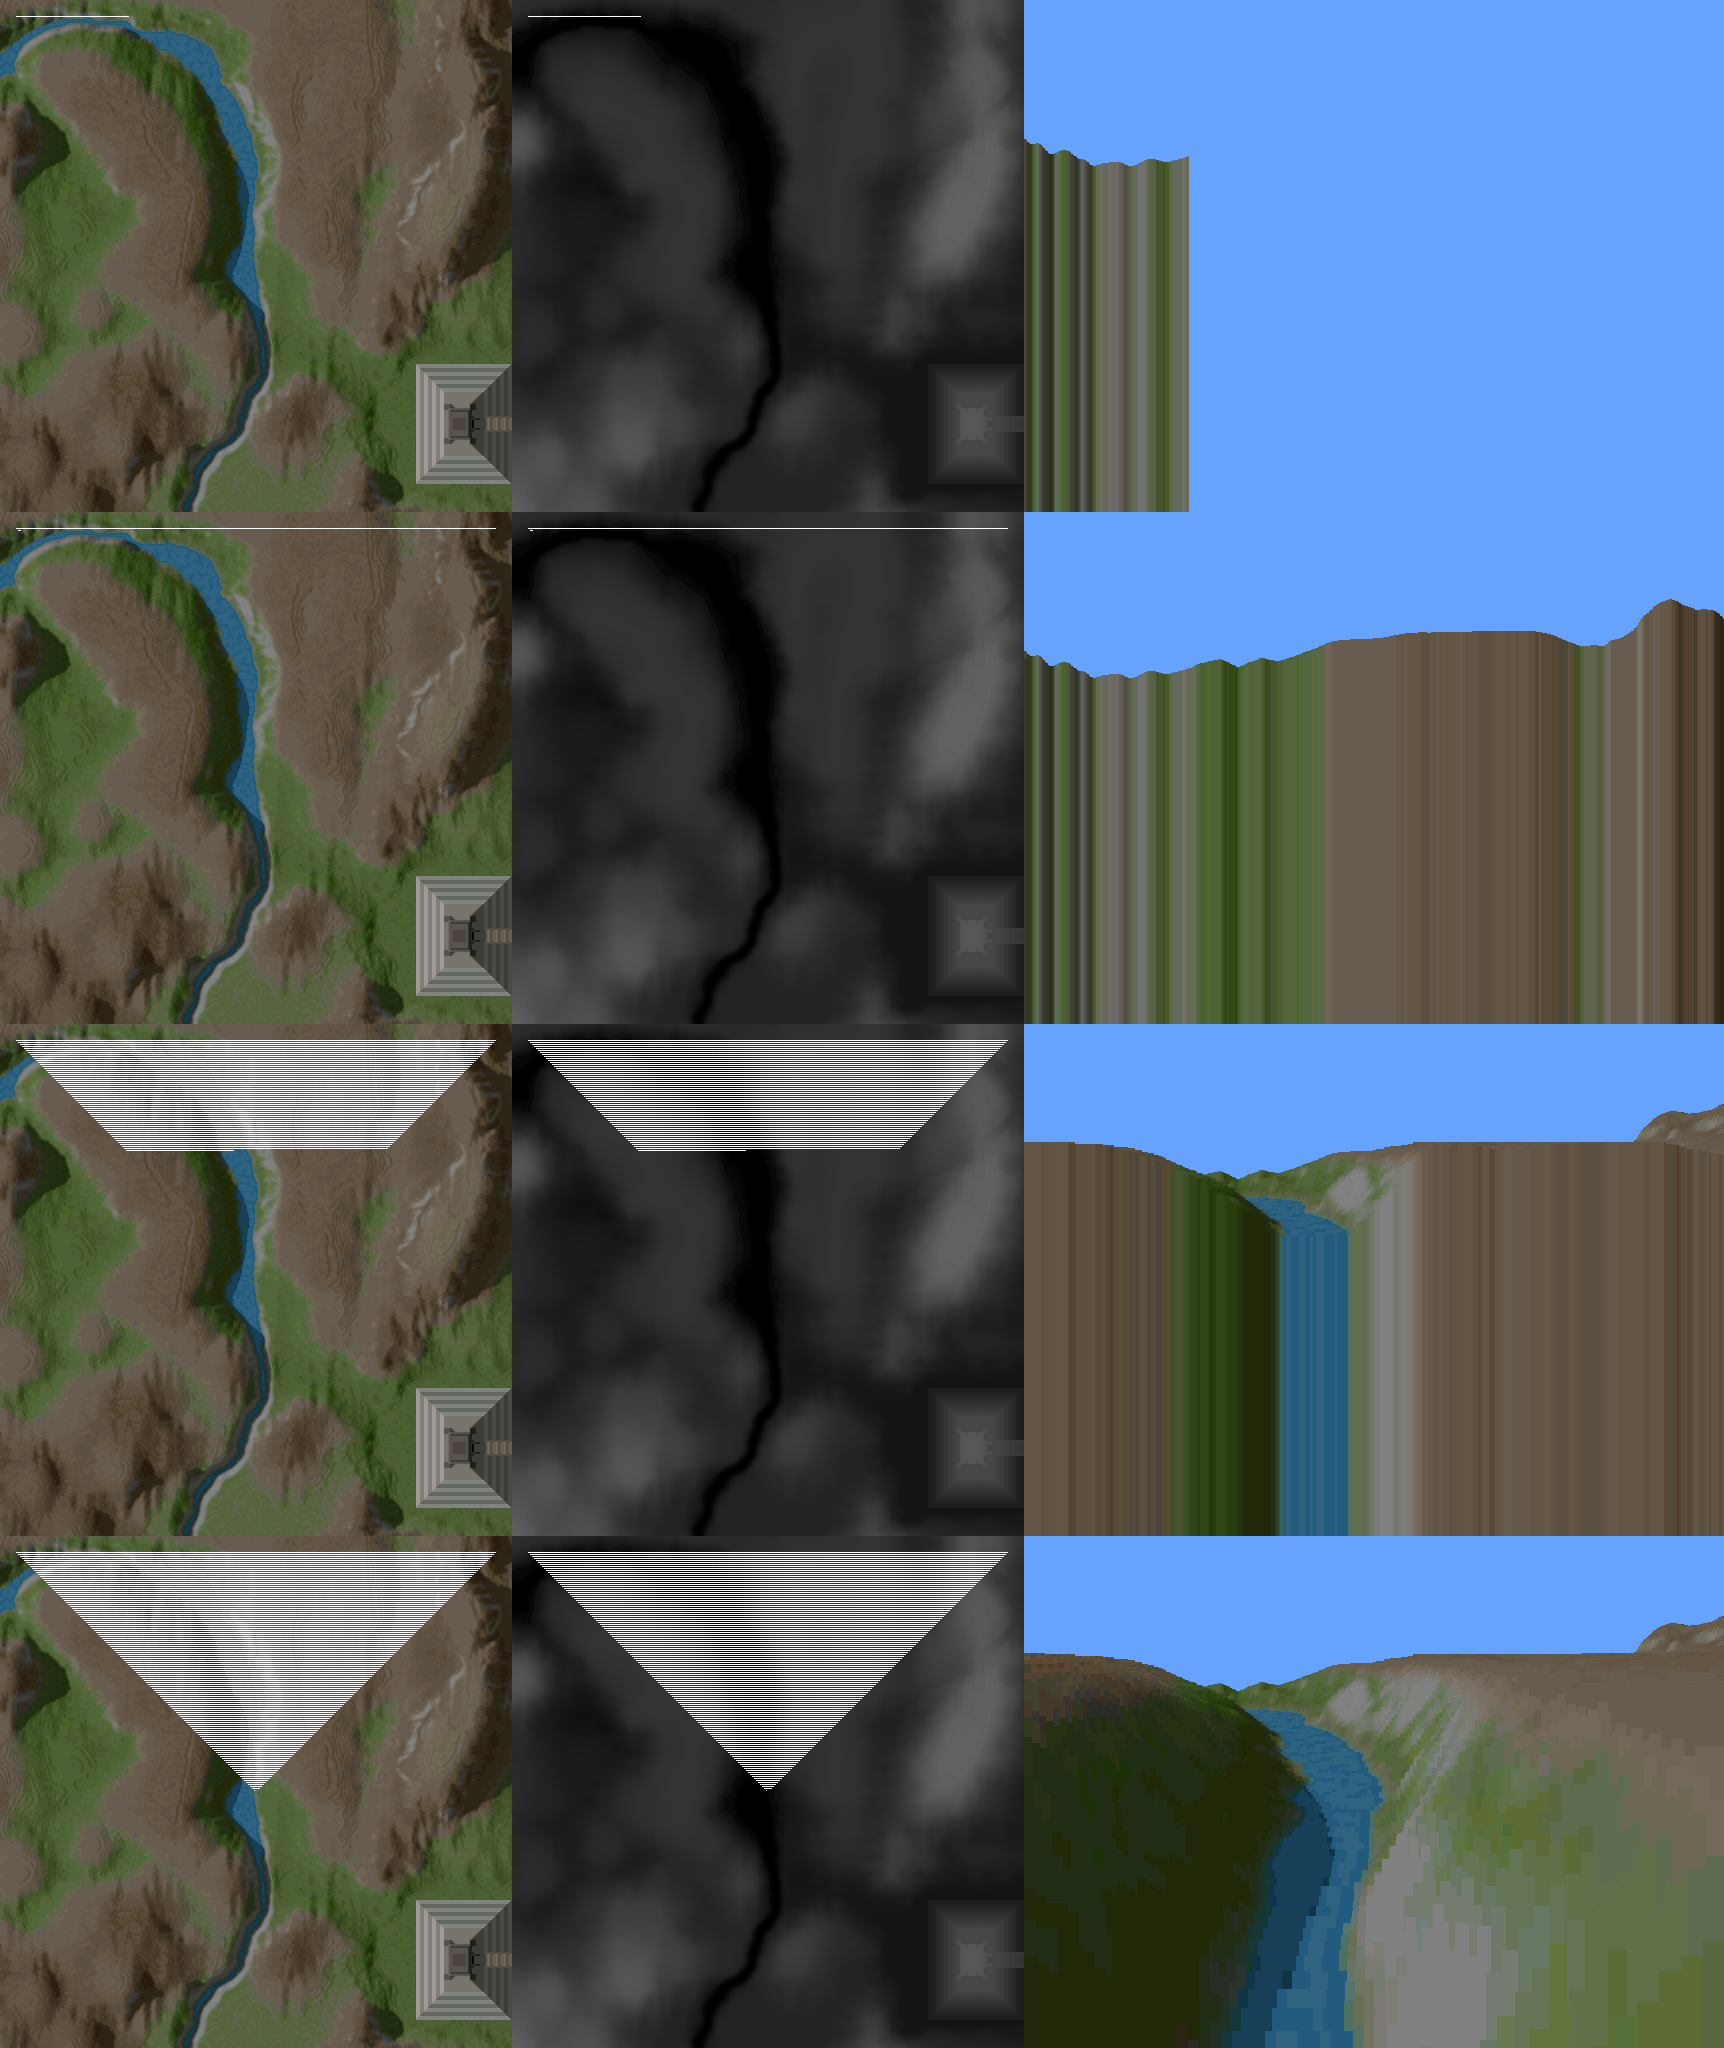
\includegraphics[scale=.2]{line-by-line}
			\captionof{figure}{Basic rasterization technique of the Voxel Space Engine. \cite{voxel-space}}
			\label{fig:fig1}
		\end{minipage}
	
		This can be optimized with drawing from front-to-back with the addition of a y-buffer in order to determine the highest y position to draw. However, the voxel-space rendering system has a downside of having fewer pixels to determine the colors and heights of closer landmasses. This creates a pixellated effect for the foreground, while the background is rendered in higher detail. This method can be seen in more detail in Figure 2. 
		 
		\begin{minipage}{\textwidth}
		 	\centering
		 	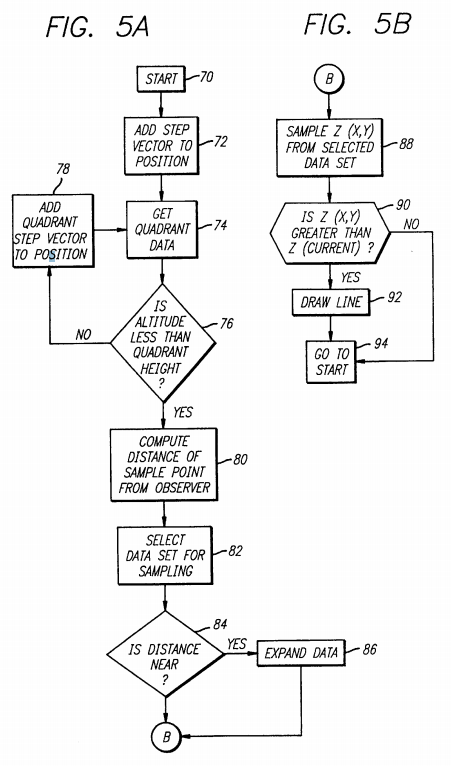
\includegraphics[scale=0.5]{US6020893A}
		 	\captionof{figure}{US Patent 6 020 893 \cite{US6020893}}
		 	\label{fig:fig10}
		\end{minipage}
		
		This weakness can be mitigated in some effect by having multiple heightmaps of differing detail to draw from. This would mitigate some of the advantage of voxel space rendering in increasing the rendering time and processing required for the algorithm. In addition to the weakness in rendering closer objects, height maps are also unable to render more complex geological formations, such as caves, archways or overhangs. Later iterations of the voxel space rendering engine worked around some of these limitations by introducing rendering of both polygons and voxels. Another possible workaround to the low resolution of the voxel space rendering system would be using procedurally generated noise as the platform for creating height maps. By creating the height map dynamically from noise, the memory used for storing the program overall would be smaller, and the resolution would not be constrained, as for areas closer to the camera, the interpolation between the points of the noise map would just be decreased. 
	
	\vspace{10pt}
	\let\clearpage\relax
	\chapter{Height Maps}
	
		As mentioned previously, Perlin noise can be used to generate height maps in order to pseudo-randomly create geological formations. While height-maps have the advantage of being two-dimensional and less complicated to run, they have difficulty in rendering a variety of geological formations. Due to the two-dimensional nature of a height map, they are unable to render more complex features such as alcoves, arches, and any other three-dimensional feature. In terms of randomness, this can create a sort of uniformity in geometry, where the only features are hills and valleys. In signal terms, this means that noise is band-limited, where almost all of the energy of the noise is concentrated in a very small part of the frequency spectrum. An example of this would be imagining an image with only black or white squares, then that same image with a guassian kernel applied to it. The high and low frequencies of the original image would be blended out, and only the band-limited output image would remain, where the high and low frequencies contribute less to the total energy \cite{making-noise}. This can be mitigated to some extent by the use of layering differing octaves of noise in order to increase the amount of variation given by the noise. 
		
		The original implementation of Perlin noise was to create representations of various textures for objects, as well as representations of clouds, fire, water and stars among other things \cite{10.1145/325165.325247}. The computation of this noise in three-dimensions is determined by computing the pseudo-random gradient at the eight nearest vertices on an integer cube. In other words, given an input point P, look at the surrounding points on the grid. In one dimension, this would be a series of line segments. 
		
		% might need to be replaced
		\begin{minipage}{\textwidth}
			\centering
			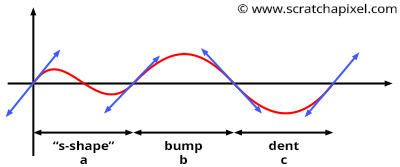
\includegraphics[scale=.5]{noise-value-vs-perlin3}
			\captionof{figure}{Perlin Noise gradients in one dimension \cite{pn-2}}
			\label{fig:fig25}
		\end{minipage} 
		
		In two-dimensions there will be four points, due to the surrounding unit square, in three-dimensions there will be eight, due to the surrounding unit cube. Similarly to how in two dimensions space is parameterized by a lattice of integer squares, in three-dimensional space it is parameterized by a series of cubes. As Perlin noise scales up, this hypercube grows larger and larger in complexity, increasing the run time. For each of these surrounding grid points, Q, a pseudo-random gradient vector, G is chosen. This gradient is pseudo-random because, while the initial determination of the gradient vector's value is randomized, when inputting the same grid point the same gradient vector is chosen. In the calculation of Perlin noise, all of the points on the grid are located at zero. This attribute of Perlin noise can be seen in Figure \#. From there, the inner product is calculated between all of the surrounding grid points, the chosen point, and the gradient vectors. This results in G * (P - Q), giving 2\textsuperscript{n} values, where n represents the dimensionality of the grid. Then, interpolate between the values down to P, using an S-shaped cross-fade curve to weigh the interpolation in each dimension. This equation is shown below.
		
		\begin{lstlisting}[language=C]
			/* 3t^2 - 2t^3 */
			define s_curve(t) ( t * t * (3. - 2. * t) )
		\end{lstlisting}
		% cite? https://mrl.cs.nyu.edu/~perlin/doc/oscar.html#noise
	
		This was the original equation used for Perlin noise, but has since been superceeded. One of the problems with the previous equation used was that the second derivative of the function, \textbf{6-12t} is not zero at either \textbf{t=0} or \textbf{t=1}, causing discontinuities in the noise. Some of the effects of this are shown in Figure \#. This led to the equation shown below to be used. 
		
		\begin{lstlisting}[language=Java]
			// 6t^5 - 15t^4 + 10t^3
			static double fade(double t) { return t * t * t * (t * (t * 6 - 15) + 10); }
		\end{lstlisting}
		% cite? https://mrl.cs.nyu.edu/~perlin/noise/
	
		This new equation led to an approximate ten percent speed increase compared to the original implementation. 
		
		\begin{minipage}{\textwidth}
			\centering
			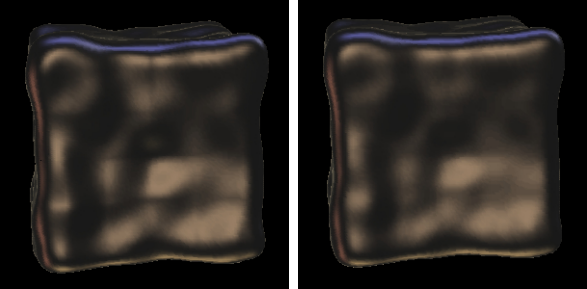
\includegraphics[scale=.5]{s-curve}
			\captionof{figure}{Removal of artifacting at t=0 and t=1 from revised interpolation function \cite{10.1145/566654.566636}}
			\label{fig:fig28}
		\end{minipage} 
		
		While Perlin noise saw great success, it was succeeded by algorithms such as Simplex noise, designed to alleviate some of the problems with Perlin noise. This included the computational complexity and the artifacting in the noise created. The artifacting in the noise appears from the necessity for the gradients to pass through zero, as shown in Figure \#. This causes unavoidable artifacting in the noise. In addition, while Perlin noise's computational complexity is acceptable when in three-dimensional space and lower, it suffers greatly from increasing the dimensionality further.
		

	\vspace{10pt}
	\let\clearpage\relax	
	\chapter{Polygons}
	
		\section{Rendering Differences}
		
		Constructing polygons from height maps, similar problem
	
	\vspace{10pt}
	\let\clearpage\relax
	\chapter{Voxels}
	
		Voxels can be used in a lot of ways to render maps 
		Talk about minecraft's storage of voxel terrain data
		Contrast with voxel rendering techniques
	
	\vspace{10pt}
	\let\clearpage\relax
	\chapter{Development}
		asd

		\section{Areas of Research}
	
		An ongoing area of research for procedural generation is the introduction of neural networks as the framework, instead of more traditional algorithms or techniques. One example of this is the procedural generation of terrain via Tensorflow. This impementation was trained on a large dataset of terrain hiehgt maps, around 10,000, with the addition of sattelite data to use for coloring. The specific neural network involved in the implementation was a Generative Adversarial network, which works on creating fake images, and attempting to discern between real and fake. By iterating this, the network will get better at both tasks, with the generator learning how to create more and more realistic images. For the problem of coloring the terrain, a style network was used to take two images and blend them in order to create an output image that looks like the content image, but with the style of the reference image. This technique is used in other applications, such as the neural networks trained on recreating photographs in a particular artist's style, shown in Figure 4. 
		
		\begin{minipage}{\textwidth}
			\centering
			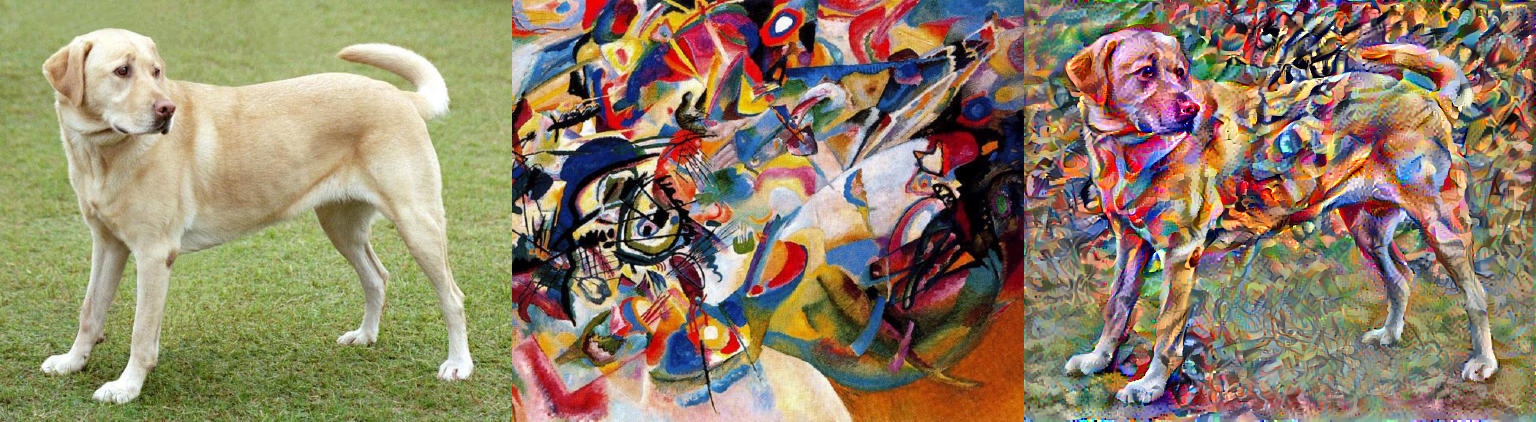
\includegraphics[scale=.3]{stylized-image}
			\captionof{figure}{An example of neural style transfer \cite{tf-style}}
			\label{fig:fig5}
		\end{minipage}
	
		
		
		\cite{Liu_2020}
		
		\section{Algorithm Advancements}
		
		Perlin noise was designed to address some of the limitations of the original Perlin noise. Since the original implementation of Perlin noise was constrained by the lattice gradient function creating directional artifacts, one of the goals of Simplex noise was to overcome this limitation. In addition, Simplex noise has lower computational complexity - O(k\textsuperscript{2}) instead of O(2\textsuperscript{k})\cite{sheet-simplex}. Other benefits includes the capability to scale to higher dimensions, a well-defined and continuous gradient, as well as simpler implementation. Instead of the lattice gradients that Perlin noise works on, Simplex noise works based on simplex grids for which it was named after. This involves choosing the simplest, repeatable shape to fill a N-dimensional space. Another definition of a n-simplex would be it being the smallest figure that contains n+1 given points in n-dimensional space, while not lying in the space of a lower dimension. In one dimension, this works by choosing repeating line segments. In two dimensions, this becomes an equilateral triangle. In three dimensions, this becomes a trianglular pyramid, also known as a tetrahedron. From four dimensions and onward, this simplex becomes increasingly difficult to visualize. However, there is a pattern in the drawability of simplexes, by creating a new point and connecting it to all previously existing points.
		
		\begin{minipage}{\textwidth}
			\centering
			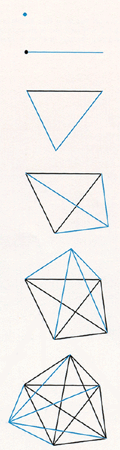
\includegraphics[scale=.75]{six simplexes}
			\captionof{figure}{The first six simplexes \cite{higher-dim-simplexes}}
			\label{fig:fig2}
		\end{minipage}
	
		The relative simplicity of the simplex shape in having as few corners as possible makes it a lot easier to interpolate values in the interior of the shape, relative to the hypercubes used in the original Perlin noise.
		In the original Perlin noise function, derivatives were used to compute the gradation between the points. This creates a large increase in computational complexity based on dimensionality. Simplex noise instead uses the summation of kernel values in order to determine the point's value. To generate the Simplex noise, the value for any point in space must be determined. In two dimensional space, this means skewing the coordinate space along the main diagonal, transforming the squashed equilateral triangles into right-angle isosceles triangles. From there, determining the location is made more simple, as just the integer part of the coordinates is needed for each dimension. Beyond two dimensions, the visualization becomes more difficult, but the methods remain the same.  
		
		\begin{minipage}{\textwidth}
			\centering
			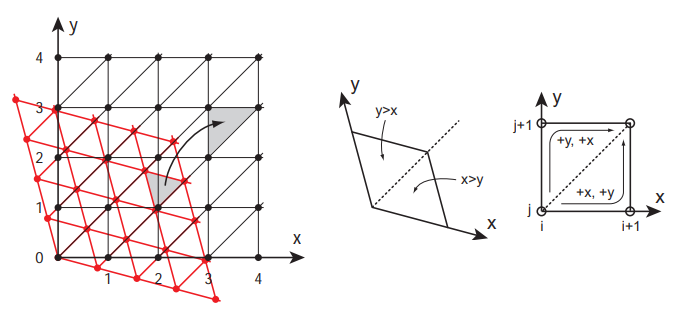
\includegraphics[scale=.5]{skewed grid}
			\captionof{figure}{Skewing in two-dimensional space and determining the cell containing a point. \cite{simplex-demyst}}
			\label{fig:fig3}
		\end{minipage}
		
		The traversal scheme for a two-dimensional simplex is built around this triangular method. If the x and y coordinates are known, then all that is needed is to determine which of the two simplices the point lies in. If x > y, the corners become (0,0), (1,0) and (1,1), else the corners are (0,0), (0,1) and (1,1). To traverse this, only one step in the x and one step in the y is needed, but in a different order for each of the simplices. This technique can then be generalized to any arbitrary amount of N dimensions \cite{simplex-demyst}. While Perlin noise has many advantages over the classical Perlin noise, it has a different visual characteristic, making it difficult to directly replace or compare the two. 
		
		\begin{minipage}{\textwidth}
			\centering
			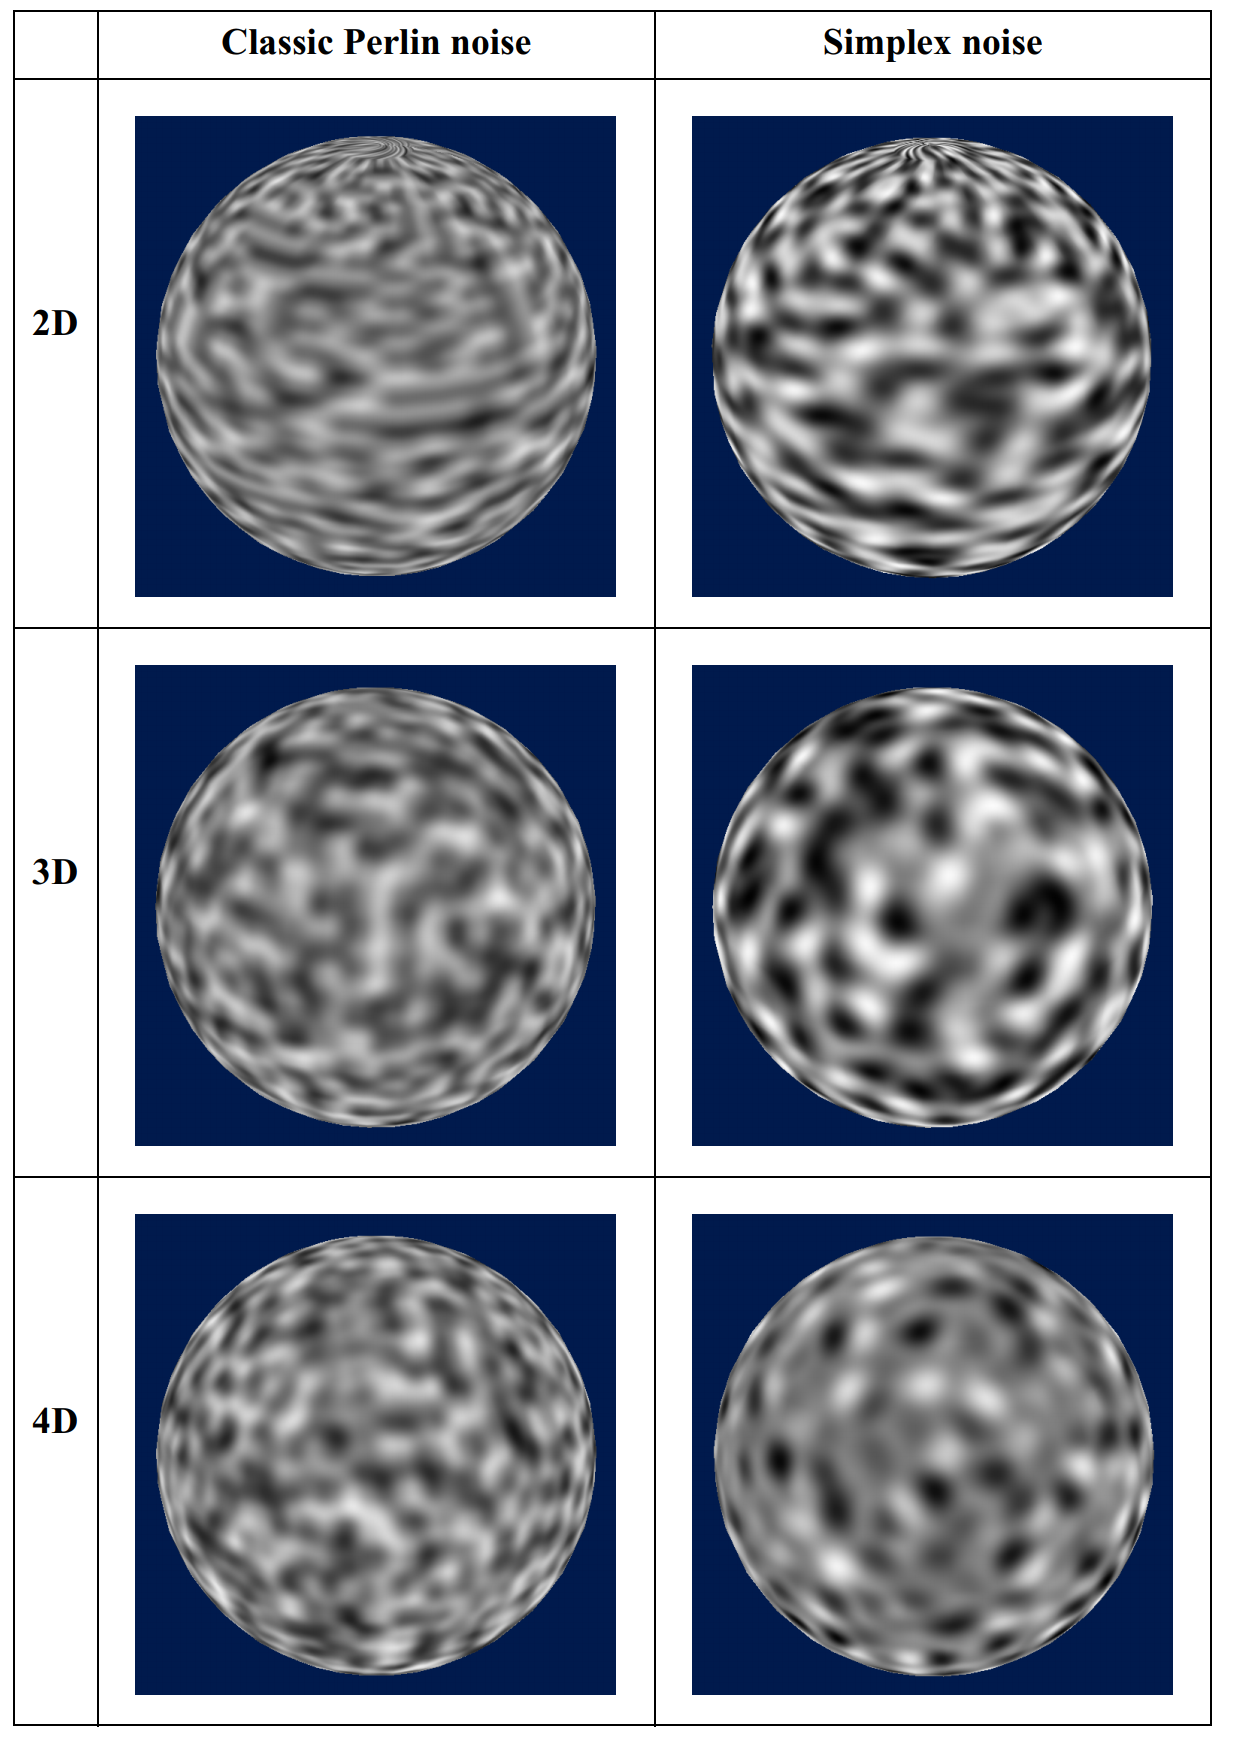
\includegraphics[scale=.25]{perlin vs simplex}
			\captionof{figure}{A comparison of Perlin and Simplex noise \cite{simplex-demyst}}
			\label{fig:fig4}
		\end{minipage}
	
		However, with additional modification using multiple layers or octaves, Simplex noise will run much more computationally efficiently, as well as replicating the visual quirks of Perlin noise. 
			
	\vspace{10pt}
	\let\clearpage\relax
	\chapter{Summary}
		
		\section{Algorithm Advancements}
		
		Perlin noise was designed to address some of the limitations of the original Perlin noise. Since the original implementation of Perlin noise was constrained by the lattice gradient function creating directional artifacts, one of the goals of Simplex noise was to overcome this limitation. In addition, Simplex noise has lower computational complexity - O(k\textsuperscript{2}) instead of O(2\textsuperscript{k})\cite{sheet-simplex}. Other benefits includes the capability to scale to higher dimensions, a well-defined and continuous gradient, as well as simpler implementation. Instead of the lattice gradients that Perlin noise works on, Simplex noise works based on simplex grids for which it was named after. This involves choosing the simplest, repeatable shape to fill a N-dimensional space. Another definition of a n-simplex would be it being the smallest figure that contains n+1 given points in n-dimensional space, while not lying in the space of a lower dimension. In one dimension, this works by choosing repeating line segments. In two dimensions, this becomes an equilateral triangle. In three dimensions, this becomes a trianglular pyramid, also known as a tetrahedron. From four dimensions and onward, this simplex becomes increasingly difficult to visualize. However, there is a pattern in the drawability of simplexes, by creating a new point and connecting it to all previously existing points.
		
	\vspace{10pt}
	\let\clearpage\relax
	\chapter{Appendix}
		filler
		
	\vspace{10pt}
	\let\clearpage\relax
	\chapter{References}
		filler
	
	\bibliographystyle{plain} % We choose the "plain" reference style
	\bibliography{refs} % Entries are in the "refs.bib" file
		
\end{document}